\chapter{AURA-MAS: System Design}
\label{chap:design}

\section{Introduction}

This chapter presents the design of AURA-MAS, from global architecture down to message schemas and coordination protocols. The design is governed by five principles derived from the analysis of Chapters~\ref{chap:background_mas}--\ref{chap:sota}:

\begin{enumerate}
    \item \textbf{Edge-first}: raw sensor data is processed where it is produced and never leaves the edge agent;
    \item \textbf{Events, not streams}: all inter-agent communication consists of small structured messages;
    \item \textbf{Deterministic decisions}: alerts are produced exclusively by an auditable rule-based policy engine;
    \item \textbf{Guarded generativity}: \gls{llm}/\gls{vlm} components explain decisions but can never make or alter them;
    \item \textbf{Privacy by design}: anonymization, minimization, and auditability are structural, not optional.
\end{enumerate}

\section{Global Architecture}

AURA-MAS is a hierarchical \gls{mas} organized in three layers connected by a two-tier message substrate (Figure~\ref{fig:architecture}).

\begin{figure}[H]
    \centering
    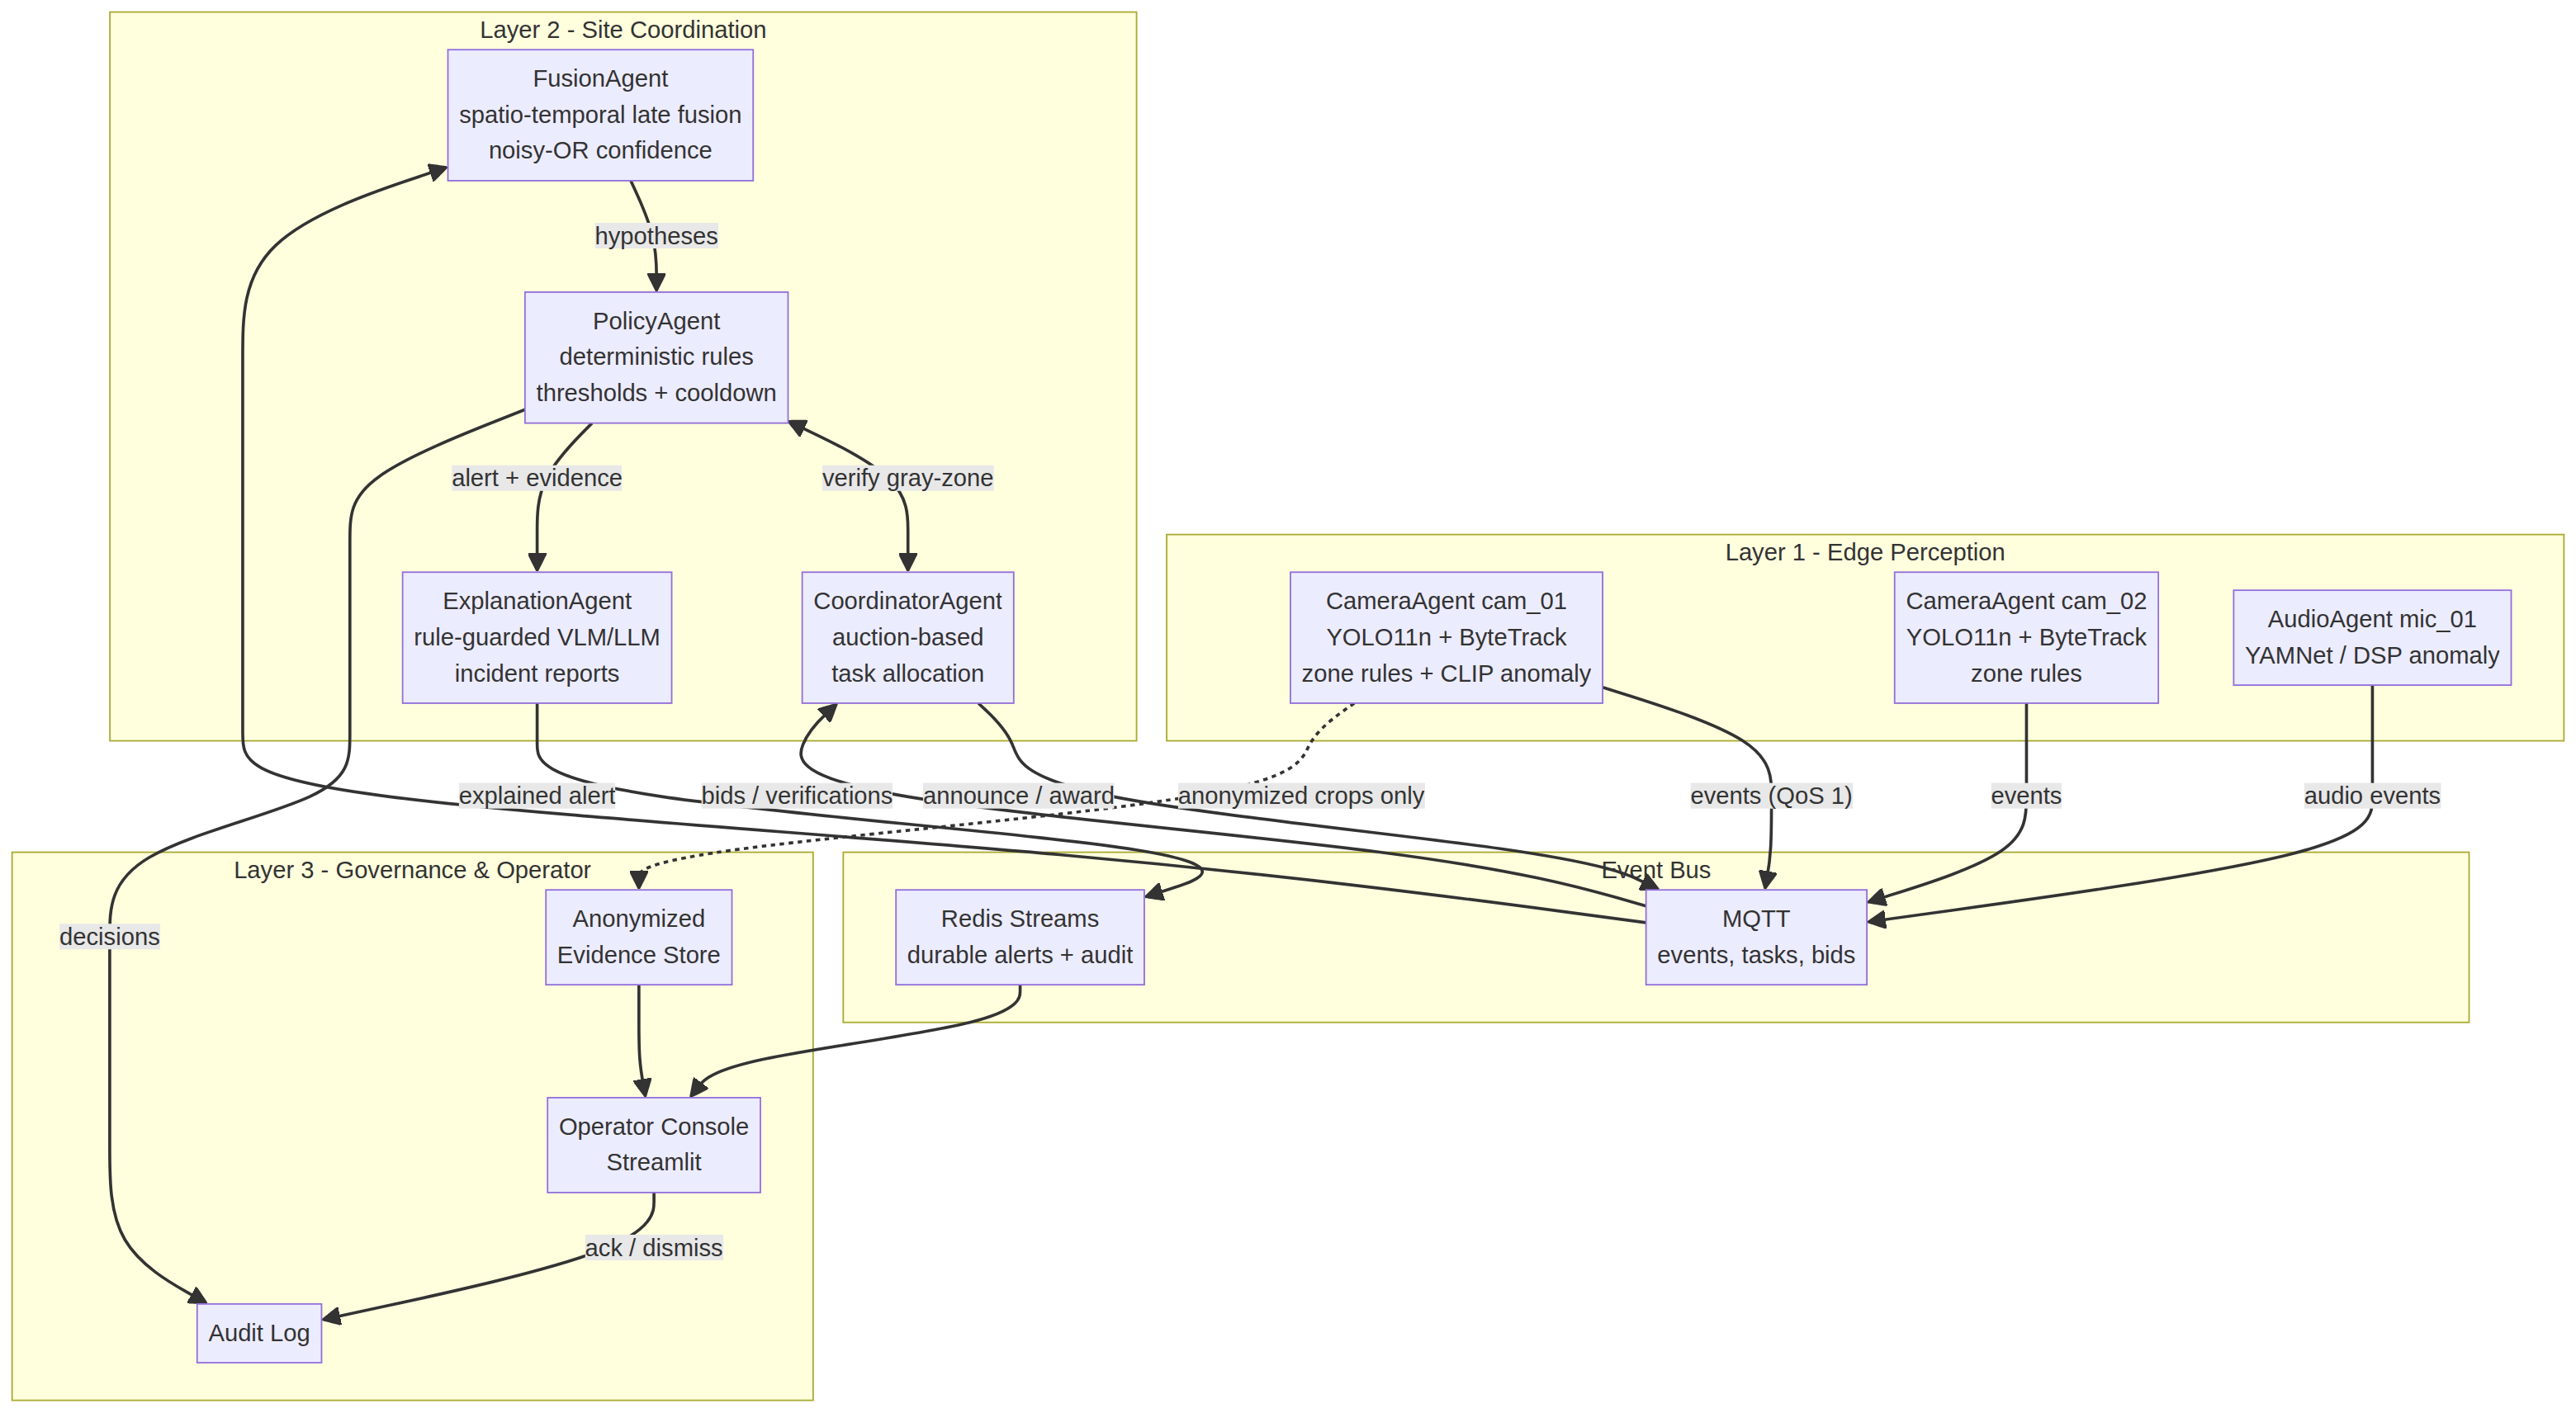
\includegraphics[width=0.98\textwidth]{Assets/fig_architecture.png}
    \caption{AURA-MAS architecture: edge perception layer, site coordination layer, and governance/operator layer, connected by an MQTT event bus and a Redis durable stream.}
    \label{fig:architecture}
\end{figure}

\textbf{Layer 1: edge perception.} One agent handles each sensor. \emph{CameraAgents} run detection, tracking, zone rules, and optional semantic anomaly scoring on their video stream. \emph{AudioAgents} classify sound events or score acoustic anomalies. Both publish structured events on the bus.

\textbf{Layer 2: site coordination.} The \emph{FusionAgent} groups events into incident hypotheses. The \emph{CoordinatorAgent} allocates verification tasks when a hypothesis is uncertain. The \emph{PolicyAgent} applies deterministic alert or suppression rules. The \emph{ExplanationAgent} produces a report for an accepted alert.

\textbf{Layer 3: governance and operator.} A web console shows alerts, anonymized evidence, and explanations. Operator actions and policy decisions are appended to the audit log. The log is append-only by convention, not cryptographically immutable.

The substrate pairs \gls{mqtt} \cite{light2017mosquitto} for low-latency fan-out of high-frequency messages (detections \gls{qos}~0; events, tasks, bids, awards \gls{qos}~1) with Redis Streams for durable, replayable storage of alerts and audit records. A single-process in-memory bus with identical semantics supports development and testing.

\section{Agent Roles and Responsibilities}

\begin{table}[H]
\centering
\caption{Agent roles in AURA-MAS.}
\label{tab:agents}
\small
\begin{tabular}{p{2.8cm}p{4.6cm}p{2.6cm}p{2.6cm}}
\toprule
\textbf{Agent} & \textbf{Responsibility} & \textbf{Consumes} & \textbf{Produces} \\
\midrule
CameraAgent & Detection, tracking, zone rules, CLIP anomaly, verification bids/execution & video frames; tasks, awards & detections, events, bids, verifications \\
AudioAgent & Sound event classification / DSP anomaly & audio chunks & events \\
FusionAgent & Spatio-temporal hypothesis formation, confidence fusion & events & hypotheses \\
CoordinatorAgent & Auction-based verification task allocation & hypotheses (gray-zone), bids, verifications & tasks, awards \\
PolicyAgent & Severity mapping, thresholds, hysteresis, alert emission, audit & hypotheses, verification results & alerts, audit records \\
ExplanationAgent & Grounded incident report generation with guardrails & alerts, hypotheses, evidence & explanations \\
Operator console & Human oversight, acknowledgment & alerts, evidence & operator audit records \\
\bottomrule
\end{tabular}
\end{table}

\section{Message Schemas}

All messages are \gls{json} documents with mandatory provenance fields. The three core schemas are:

\textbf{Detection} (high-frequency, transient): \texttt{\{sensor\_id, frame\_id, timestamp, objects: [\{class, confidence, bbox, track\_id\}]\}}.

\textbf{Event} (semantic, durable): \texttt{\{event\_id, sensor\_id, timestamp, event\_type, confidence $\in [0,1]$, modality, zone, track\_id, evidence\_path, extra\}}. Event types include \texttt{intrusion}, \texttt{loitering}, \texttt{abandoned\_object}, \texttt{anomaly}, and audio types (\texttt{audio\_glass\_break}, \texttt{audio\_scream}, \ldots). The \texttt{evidence\_path} always references an \emph{anonymized} crop.

\textbf{Alert} (operator-facing): \texttt{\{alert\_id, timestamp, severity $\in$ \{CRITICAL, WARNING, INFO\}, event\_type, confidence, zone, sensors[], evidence[], fused\_events[], explanation, status\}}.

\section{Edge Perception Design}

\subsection{Camera Pipeline}

Each CameraAgent samples its stream at a configurable inference rate (default 5~\gls{fps}) and runs a four-stage pipeline: (1) YOLO11n detection with ByteTrack association \cite{ultralytics2025yolov8, zhang2022bytetrack}; (2) a stateful \emph{zone rule engine} evaluating declarative site rules; (3) optional \gls{clip} zero-shot anomaly scoring on subsampled frames \cite{radford2021clip}; (4) event emission with anonymized evidence.

The zone rule engine implements three rules over tracked objects, using the foot point (bottom-center of the bounding box) for zone membership tested by ray-casting against declared polygons:

\begin{itemize}
    \item \textbf{Intrusion}: a \texttt{person} track enters a zone declared \texttt{restricted}; fired once per (track, zone) pair.
    \item \textbf{Loitering}: dwell time of a person track inside any zone exceeds a threshold $\tau_{loiter}$ (default 8~s); confidence grows with dwell time.
    \item \textbf{Abandoned object}: a non-person track remains static (\gls{iou} with its initial box $> 0.6$) longer than $\tau_{aband}$ (default 10~s).
\end{itemize}

\subsection{Audio Pipeline}

AudioAgents process audio in overlapping windows extending up to 1.5~s of lookback context per 1-second chunk, so that short transient sounds are scored with sufficient temporal context rather than against a bare 1~s window. In YAMNet mode\footnote{The \gls{dsp} fallback triggers not only when \texttt{tensorflow}/\texttt{tensorflow\_hub} are absent, but also transiently on model-load failure; an earlier silent \texttt{except Exception} around the YAMNet load masked a dead model URL for an unknown period, motivating an explicit \texttt{backend="yamnet"} configuration option that now fails loudly instead of silently falling back.} \cite{tensorflow_yamnet}, a curated mapping from AudioSet classes to surveillance event types (with per-class thresholds) produces typed events. In \gls{dsp} fallback mode, rolling z-scores of short-time energy and spectral flatness produce generic \texttt{audio\_anomaly} events, normalized to $[0,1]$.

\section{Fusion Design}
\label{sec:design_fusion}

The FusionAgent maintains a set of open \emph{hypotheses}, keyed by (incident family, zone), where families group mutually corroborating event types (e.g., \texttt{intrusion} and \texttt{audio\_glass\_break} both belong to \emph{security}). An incoming event either joins the open hypothesis for its key (if within the sliding window $W$, default 6~s, of the last event) or opens a new one.

Hypothesis confidence uses a reliability-weighted noisy-OR:
\begin{equation}
    C(H) = 1 - \prod_{e \in H} \bigl(1 - w_{m(e)} \cdot c_e\bigr) \;+\; \beta_{mod} \cdot \mathbb{1}[|M(H)|>1] \;+\; \beta_{sen} \cdot \mathbb{1}[|S(H)|>1]
\label{eq:noisyor}
\end{equation}
where $c_e$ is event confidence, $w_{m}$ a per-modality reliability weight (video 0.9, audio 0.7), $M(H)$ and $S(H)$ the sets of modalities and sensors contributing to $H$, and $\beta_{mod}=\beta_{sen}=0.05$ small corroboration bonuses; the result is clamped to $[0,1]$. The noisy-OR form guarantees monotonicity: additional supporting evidence never decreases confidence, and independent corroboration from a second modality or sensor strictly increases it---the formal core of contribution C3. When a hypothesis window closes, the hypothesis is flushed to the PolicyAgent.

\section{Coordination Design}
\label{sec:design_coordination}

Fused confidence in the \emph{gray zone} $[\theta_{lo}, \theta_{hi})$ (defaults $0.35$--$0.75$) means the system is neither confident enough to alert nor to dismiss. Rather than guessing, the CoordinatorAgent buys information through a single-round sealed-bid auction derived from the \gls{cnp} \cite{smith1980contract}:

\begin{enumerate}
    \item \textbf{Announce}: the coordinator publishes a verification task $\langle$task\_id, event\_type, zone, origin\_sensor$\rangle$ on the task topic.
    \item \textbf{Bid}: each CameraAgent computes a private utility $u = b \cdot \kappa \cdot o$ where $b$ penalizes the origin sensor (0.3 vs 1.0, favoring independent confirmation), $\kappa$ reflects current load (0.2 if busy), and $o \in [0,1]$ is its field-of-view overlap with the event zone; it publishes the bid within the bidding window $T_b$ (default 1~s).
    \item \textbf{Award}: the coordinator awards the task to the highest bidder.
    \item \textbf{Verify}: the winner re-analyzes its current frame at higher scrutiny (larger input resolution, lower confidence floor) and reports \texttt{verified} with a verification score.
    \item \textbf{Integrate}: the PolicyAgent adjusts hypothesis confidence: $+0.15$ if verified, $-0.20$ if refuted.
\end{enumerate}

The protocol costs $O(n)$ messages per task ($n$ = number of cameras) and bounded wall time $T_b + T_{verify}$. A round-robin allocator (ignoring utilities) serves as the ablation baseline, and coordination can be disabled entirely.

\begin{revisionbox}
The utility expression states the intended design, but the v2 campaign did not
populate \texttt{fov\_overlap} in its manifests. During those measurements,
$o$ consequently used the 0.5 fallback for every camera. The reported campaign
does not validate spatially informed bidding; the correction and its evidence
are discussed in Section~\ref{sec:c2_retraction}.
\end{revisionbox}

\section{Policy and Alerting Design}

The PolicyAgent is the sole component authorized to create alerts. Its decision procedure is fully deterministic: (1) map the hypothesis's dominant event type to a severity class (e.g., \texttt{intrusion} and \texttt{audio\_gunshot} $\rightarrow$ CRITICAL; \texttt{loitering} $\rightarrow$ INFO); (2) optionally request verification for gray-zone confidence; (3) compare adjusted confidence to a per-severity threshold (CRITICAL 0.45, WARNING 0.55, INFO 0.70---lower thresholds for higher-stakes events reflect asymmetric miss costs); (4) apply per-(zone, type) cooldown (default 20~s) to prevent alert storms; (5) write \emph{every} decision---alert or suppression, with reason---to the audit stream. This design directly implements the human-oversight and logging obligations of high-risk AI systems under the EU AI Act \cite{euaiact2024}.

\section{Agentic Explanation Design}

The ExplanationAgent runs a small state machine (collect evidence $\rightarrow$ describe frames with a \gls{vlm} $\rightarrow$ draft structured report $\rightarrow$ guardrail check), implementable in LangGraph \cite{langgraph2024} or directly. The system prompt constrains the model to use only supplied evidence, cite evidence by exact identifiers, avoid identity speculation, and recommend only observation actions. The \emph{guardrail} then mechanically verifies that (a) the output parses to the required \gls{json} schema and (b) every cited evidence identifier---in the citation list and in free text---exists in the hypothesis event log. Any violation triggers fallback to a deterministic template that is always available. Because the alert has already been emitted when explanation begins, generation latency and failures affect only report richness, never safety (contribution C4).

\section{Privacy and Governance by Design}

Table~\ref{tab:privacy} maps regulatory requirements to design mechanisms.

\begin{table}[H]
\centering
\caption{Privacy-by-design mechanisms in AURA-MAS.}
\label{tab:privacy}
\small
\begin{tabular}{p{4.5cm}p{8.5cm}}
\toprule
\textbf{Requirement (GDPR / AI Act)} & \textbf{Mechanism} \\
\midrule
Data minimization & Only \gls{json} events cross the network; raw frames never leave the edge agent \\
No biometric identification & No face recognition or \gls{reid}; corroboration at event level only \\
Anonymization & All exported evidence passes through person/face blurring; fail-closed (full-frame blur if localization unavailable) \\
Storage limitation & Evidence retention window configurable; detections are transient (\gls{qos} 0, not persisted) \\
Human oversight & Operator console with acknowledge/dismiss authority; no automated enforcement actions \\
Logging \& traceability & Append-only audit stream of every policy decision and operator action; cryptographic immutability is not implemented \\
Transparency & Grounded natural-language explanations with verifiable evidence citations \\
\bottomrule
\end{tabular}
\end{table}

\section{Conclusion}

AURA-MAS assigns perception to sensor-local agents, uses an auction for uncertain verification, keeps alert decisions in a deterministic policy engine, and places generative AI after the decision. The next chapter describes the implementation.
